\documentclass{beamer}

\mode<presentation> {
\usetheme{Malmoe} 
\usecolortheme{beaver} 
}

\usepackage{graphicx} 
\usepackage{booktabs} 
\usepackage{amsmath}
\usepackage{graphicx}
\usepackage[colorinlistoftodos]{todonotes}
\usepackage{hyperref}
\usepackage{multimedia}
\usepackage{media9}
\usepackage{tikz}
\usetikzlibrary{calc,positioning}
\usepackage{xcolor}
\hypersetup{
    colorlinks=true,       
    linkcolor=blue,          
    citecolor=blue,        
    urlcolor=blue           
}
%----------------------------------------------------------------------------------------
%	TITLE PAGE
%----------------------------------------------------------------------------------------

\title[CPS]{\textcolor{black}{{Consensus and cooperation in networked multi-agent systems \cite{p1}}}} 
\subtitle[]{}

\author{George Kontoudis, DevaPrakash Muniraj}
\institute[VT] 
{Homework 2\\
AOE5984 Cyber-Physical Systems and Distributed Control\\
Spring 2017\\
\medskip
\it{Aerospace and Ocean Engineering Department, Virginia Tech} 
}
\date{\today}

\setbeamertemplate{footline}[text line]{%
  \parbox{\linewidth}{\vspace*{-8pt}\today 
  \hfill\insertshortsubtitle
  \hfill\insertpagenumber}}
\setbeamertemplate{navigation symbols}{}

\begin{document}

\begin{frame}[plain]
\titlepage 
\end{frame}

\begin{frame}
\frametitle{Outline} 
\tableofcontents 
\end{frame}

%----------------------------------------------------------------------------------------
%	PRESENTATION SLIDES
%----------------------------------------------------------------------------------------
%------------------------------------------------
\section{Introduction}
%------------------------------------------------

\begin{frame}
\frametitle{Consensus \& Cooperation}
This paper provides a framework for analysis of consensus algorithms for multi-agent network systems
\begin{itemize}
\item Consensus is defined as reaching an agreement regarding a certain quantity of interest that depends on the state of all agents \vspace{0.2cm}
\item A protocol, also called consensus algorithm, is an interaction rule that specifies the exchange information between an agent and its neighbors on the network\vspace{0.2cm}
\item Networked systems, that are included in agents, are equipped with sensing, computing, and communicating devices
\end{itemize}
\end{frame}

%------------------------------------------------

\begin{frame}
\frametitle{Consensus in Networks}
\begin{itemize}
\item For a directed graph $G=(V,E)$, with a set of nodes $V={1,2,...,n}$ and edges $E \subseteq V \times V$. A simple consensus algorithm of a $n$th order linear system on a graph is 
\begin{equation*}
\dot{x}_i = \sum_{j \in N_i}(x_j(t)-x_i(t))+b_i(t), \hspace{0.2cm} x_i(0)=z_i \in \mathbb{R}, b_i(t)=0
\end{equation*}
with collective dynamics
$\dot{x} = -Lx$
\item Since all row-sums of the Laplacian are zero, L has always a zero eigenvalue $\lambda_1=0$
\item The consensus value is the avg of the initial states $\alpha=\frac{1}{n}\sum_i z_i$
\end{itemize}
\end{frame}

%------------------------------------------------

\begin{frame}
\frametitle{The $f$-Consensus problem \& Cooperation}
Differences between constrained and unconstrained problems
\begin{itemize}
\item In unconstrained problems the state of all agents asymptotically become the same  
\item In constrained problems (f-consensus problems) the state of all agents asymptotically become $f(z)$ 
\end{itemize}
\vspace{0.2cm}
To solve the $f$-consensus problem we need 
\begin{itemize}
\item Willingness to participate from all agents
\item Cooperation from all agents
\end{itemize}
\end{frame}

%------------------------------------------------

\begin{frame}
\frametitle{Applications (1/2)}
Common consensus problems for multi-agent systems
\begin{itemize}
\item Synchronization of coupled oscillators which has dynamics
\begin{equation*}
\dot{\theta}_i = \kappa \sum_{j \in N_i}sin(\theta_j-\theta_i) + \omega_i,
\end{equation*}
where $\omega_i$ is frequency and $\theta_i$ is the phase of the $i$th oscillator
\item Flocking theory of mobile agents with sensing and communication devices, using proximity graphs
\item Fast consensus in small-worlds deals with network design problem. The problem is addressed with either design of weights or design of topology.
\end{itemize}
\end{frame}

%------------------------------------------------

\begin{frame}
\frametitle{Applications (2/2)}
\begin{itemize}
\item Rendezvous in space which reaches a consensus in position by a number of agents
\item Distributed sensor fusion in sensor networks to implement or approximate a Kalman-filter, or estimate linear least-squares
\item Distributed formation control for multi-vehicle formation are using protocols
\begin{equation*}
\dot{x}_i=\sum_{j \in N_i}(x_j-x_i-r_{ij})
\end{equation*}
where $r_{ij}$ is the desired inter-vehicle relative position vector
\end{itemize}
\end{frame}

%------------------------------------------------
\section{Information Consensus in Networked Systems}
%------------------------------------------------

\begin{frame}
\frametitle{Information Consensus in Networked Systems}
\begin{itemize}
\item Consider the dynamics $\dot{x}_i=u_i$ of a graph $G=(V,E)$, that reaches consensus asymptotically
\item The adjacency matrix is $A=[a_{ij}]$, and the set of neighbors $N_i = {j \in V : a_{ij}\ne 0}$
\item A dynamic graph is time-varying $G(t)=(V,E(t))$ with the $A(t)$ and the linear system is a distributed consensus algorithm
\begin{equation*}
\dot{x}_i(t) = \sum_{j \in N-i}a_{ij}(x_j(t)-x_i(t))
\end{equation*}
\item For undirected graphs ($a_{ij}=a_{ji}$) as $t=\infty$ results the avg of the initial states $\alpha=\frac{1}{n}\sum_i x_i(0)$
\end{itemize}
\end{frame}

%------------------------------------------------

\begin{frame}
\frametitle{Laplacian expression}
\begin{itemize}
\item A Laplacian representation of the dynamics is given by $\dot{x} = -Lx$, where $L=D-A$ \vspace{.2cm}
\item For undirected graphs the Laplcian satisfies the SoS property $x^{\intercal}Lx=\frac{1}{2}\sum_{(i,j)\in E}a_{ij}(x_j-x_i)^2$ \vspace{.2cm}
\item By setting $\frac{1}{2}x^{\intercal}Lx=\phi(x)$ we get the gradient-descent algorithm $\dot{x}=-\nabla \phi(x)$ \vspace{.2cm}
\item For an undirected graph the algorithm converges asymptotically for all initial values
\end{itemize}
\end{frame}

%------------------------------------------------
\subsection{Algebraic Connectivity \& Spectral Properties}

\begin{frame}
\frametitle{Algebraic Connectivity \& Spectral Properties}
\begin{itemize}
\item According to Gershgorin theorem, eigenvalues of the Laplacian matrix $L$ are located in a disk centered at $\Delta + 0j$ with radius $\Delta=max_i d_i$
\item $L$ is a symmetric graph w/ real eigenvalues for undirected graphs, so the $\lambda$ can be ordered as
\begin{equation*}
0=\lambda_1 \leq \lambda_2 \leq ... \leq \lambda_n \leq 2\Delta
\end{equation*}  
\item The second smallest eigenvalue $\lambda_2$ is called algebraic connectivity of a graph and measures the performance of consensus 
\end{itemize}
\end{frame}

%------------------------------------------------

\begin{frame}
\frametitle{Example of Algebraic Connectivity}
 
\begin{itemize}
\item Consider a regular network w/ 80 links
\begin{center}
 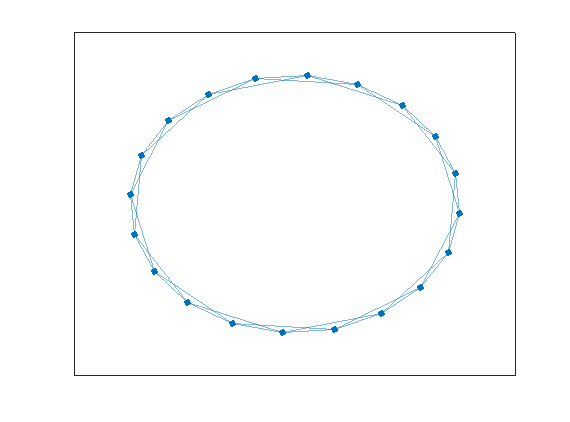
\includegraphics[width=.35\textwidth]{figures/Regular80links.png}
\end{center}
\item The Laplacian eigenvalues are
$\lambda_1=0, \lambda_2=\lambda_3=0.48, \lambda_4=\lambda_5=1.77,\lambda_6=\lambda_7=3.44
\lambda_8=4,\lambda_9=\lambda_{10}=4.28,\lambda_{11}=\lambda_{12}=\lambda_{13}=\lambda_{14}=5,\lambda_{15}=\lambda_{16}=5.79,\lambda_{17}=\lambda_{18}=6,\lambda_{19}=\lambda_{20}=6.24\leq 2\Delta=8$
\end{itemize}
\end{frame}

%------------------------------------------------
\subsection{Convergence Analysis for Directed Networks}

\begin{frame}
\frametitle{Strongly Connected and Balanced Graphs}
\begin{itemize}
\item Strongly connected graphs have a directed path that connects any two nodes
\item For a strongly connected graph $rank(L)=n-1$ and all non-trivial eigenvalues have positive real parts
\item For a strongly connected graph w/ $c\geq 1$ strongly connected components, $rank(L)=n-c$
\item Balanced graph is a digraph w/ $\sum_{j\neq i}a_{ij}=\sum_{i\neq j}a_{ji}$, which means that the total weight of edges entering and leaving a node are equal for all nodes
\item Another property of balanced digraphs is that $w=\underline{1}$ is a left eigenvector of their Laplacian, $\underline{1} ^{\intercal}L=0$
\end{itemize}
\end{frame}

%------------------------------------------------

\begin{frame}
\frametitle{Convergence Analysis}
\begin{itemize}
\item For a strongly connected digraph w/ left eigenvector $\gamma=(\gamma_1, ..., \gamma_n)$ which satisfies $\gamma^{\intercal}L=0$ and follows the consensus algorithm
\begin{equation*}
\dot{x}_i(t)=\sum_{j\in N_i}a_{ij}(x_j(t)-x_i(t)), \hspace{.2cm} x(0)=z
\end{equation*}
\item A consensus is asymptotically reached for all initial states
\item Solves the $f$-consensus problem with the linear function $f(z)=\frac{\gamma^{\intercal}z}{\gamma^{\intercal}\underline{1}}$
\item If the digraph is balanced an avg-consensus is asymptotically reached and $\alpha=\frac{\sum_ix_i(0)}{n}$
\end{itemize}
\end{frame}

%------------------------------------------------
\subsection{Consensus in Discrete-Time and Matrix Theory}

\begin{frame}
\frametitle{Discrete-Time Disrtibuted Consensus Algorithm}
\begin{itemize}
\item An iterative form of the consensus algorithm is
\begin{equation*}
x_i(k+1)=x_i(k)+\epsilon \sum_{j\in N_i}a_{ij}(x_j(k)-x_i(k))
\end{equation*}
\item Can be also formed as 
\begin{equation*}
x(k+1)=P(x(k))
\end{equation*}
\item $P$ is the Perron matrix of the graph $P=I-\epsilon L$, and $\epsilon>0$ is the step size 
\item If $\lambda_j$ is the $j$th eigenvalue of L, then $\mu_j = 1-\epsilon \lambda_j$ is the $j$th eigenvalue of P 
\end{itemize}
\end{frame}

%------------------------------------------------

\begin{frame}
\frametitle{Matrix Theory}
Three type of matrices are introduced
\begin{enumerate}
\item Irreducible  matrix if its associated graph is strongly connected \vspace{.2cm}
\item A non-negative matrix is called row (or column) stohastic if all of tis row-sums (or column-sums) are 1 \vspace{.2cm}
\item An irreducible, stohastic matrix is primitive if it has only one eigenvalue w/ maximum modulus (maximum eigenvalue has a simple root) 
\end{enumerate}
\end{frame}

%------------------------------------------------

\begin{frame}
\frametitle{Perron Matrix and Step Size Properties}
For a digraph G w/ n-nodes and maximum degree $\Delta = max_i(\sum_{j\neq i}a_{ij})$, then the Perron $P$ w/ parameters $\epsilon \in (0,\frac{1}{\Delta})$ satisfies
\begin{itemize}
\item P is row stohastic, non-negative matrix w/ trivial eigenvalue 1
\item All eigenvalues P are in the unit circle
\item If G is a balanced graph then P is a doubly stohastic graph (both row-sums and row-columns are 1)
\item If G is strongly connected and the step is $0< \epsilon <\frac{1}{\Delta}$, then $P$ is a primitive matrix. The condition $\epsilon <\frac{1}{\Delta}$ is necessary, because if the step-size is incorrect then P would no longer be a primitive matrix (multiple eigenvalues of 1)
\end{itemize}
\end{frame}

%------------------------------------------------

\begin{frame}
\frametitle{Consensus in Discrete-Time}
Consider a network of agents w/ a strongly connected digraph following the distributed network algorithm
\begin{equation*}
x_i(k+1)=x_i(k)+\epsilon \sum_{j\in N_i}a_{ij}(x_j(k)-x_i(k)),
\end{equation*}
where $0< \epsilon <\frac{1}{\Delta}$
\begin{itemize}
\item A consensus is asymptotically reached for all initial states
\item The consensus value is $\alpha = \sum_iw_ix_i(0)$, w/ $\sum_i w_i = \underline{1}$
\item If the digraph is balanced an avg consensus is asymptotically reached $\alpha=\frac{\sum_ix_i(0)}{n}$
\end{itemize}
\end{frame}

%------------------------------------------------
%\subsection{Performance of Consensus Algorithms}
%
%\begin{frame}
%\frametitle{Performance of Consensus Algorithms}
%
%
%\end{frame}

%------------------------------------------------
\subsection{Alternative Forms of Consensus Algorithms}

\begin{frame}
\frametitle{Formation Control for a Network of Multiple Vehicles CT }
\begin{itemize}
\item For a network of multiple vehicles a Laplacian-based system w/ weights $0-1$
\begin{equation*}
\dot{x}_i=\frac{1}{|N_i|}\sum_{j\in N_i}(x_j-x_i)
\end{equation*}
\item Adjacency elements are $a_{ij}=\frac{1}{|N_i|}=\frac{1}{d_i}$ for $j\in N_i$ and $0$  for $j\notin N_i$, so $d_i=\sum_{j\neq i}a_{ij}=1, \forall i$. That means the degree matrix is $D^{\ast}=I$ and the adjacency matrix is $A^{\ast}=D^{-1}A$
\item Given the dynamics $\dot{x}=-Qx$, an alternative Laplacian matrix results as $Q=D^{\ast}-A^{\ast}=I-D^{-1}A$
\end{itemize}
\end{frame}

%------------------------------------------------

\begin{frame}
\frametitle{Formation Control for a Network of Multiple Vehicles DT}
\begin{itemize}
\item For such case the Perron matrix becomes $P=I-\epsilon L^{\ast}, 0<\epsilon <1$
\item The iterative consensus algorithm 
\begin{equation*}
x(k+1)=Px(k)=[(1-\epsilon )I-\epsilon D^{-1}A]x(k)
\end{equation*}
\item If we select $\epsilon =1$ the iterative consensus algorithm becomes $x(k+1)=D^{-1}Ax(k)$, which does not converge for digraph
\item The Markov process known as random walks on a graph results for $\pi(k+1)=P\pi(k)$, w/ $\epsilon = 1$, and transition probability matrix $P=D^{-1}A$
\end{itemize}
\end{frame}

%------------------------------------------------

\begin{frame}
\frametitle{Autonomous Agents Using Nearest Neighbor Rules DT}
\begin{itemize}
\item DT consensus algorithm for undirected networks 
\begin{equation*}
x_i(k+1)=\frac{1}{1+|N_i|}(x_i(k)+\sum_{j\in N_i}x_j(k))
\end{equation*}
\item Can be also expressed as $x(k+1)=Px(k)=(I+D)^{-1}(I+A)x(k)$
\item The Perron matrix result form the normalized Laplacian $Q_l=I-(I+D)^{-1}(I+A)$
\item This algorithm is identical w/ the case of formation control for a network w/ multiple vehicles DT
\end{itemize}
\end{frame}

%------------------------------------------------

\begin{frame}
\frametitle{Different forms of Laplacians}
\begin{table}
\centering
\begin{tabular}{|c|c|c|c|}
\hline \multicolumn{4}{|c|}{\scriptsize{\textbf{Laplacian Forms}}} \\
\hline \scriptsize{\#} &  \scriptsize{Laplacian L} & \scriptsize{Perron P} & \scriptsize{\textbf{$\epsilon$}} \\
\hline \scriptsize{1} & \scriptsize{$D-A$}  & \scriptsize{$I-\epsilon L$} & \scriptsize{$(0,\Delta^{-1})$} \\
\hline \scriptsize{2} & \scriptsize{$I-D^{-1}A$}  & \scriptsize{$D^{-1}A$} & \scriptsize{1}  \\
\hline \scriptsize{3} & \scriptsize{$I-(I+D)^{-1}(I+A)$ } & \scriptsize{$(I+D)^{-1}(I+A)$} & \scriptsize{1} \\
\hline
\end{tabular}
\end{table}
\begin{itemize}
\item The algorithms in all three cases are in two forms
\begin{equation*}
\dot{x}=-Lx, \hspace{.4cm}
x(k+1)=Px(k)
\end{equation*}
\item The first and the third forms guarantee stability of a DT linear system for all possible connected networks
\item The second form needs analysis to verify P stability
\end{itemize}
\end{frame}

%------------------------------------------------
\subsection{Weighted-Average Consensus}

\begin{frame}
\frametitle{Weighted-Average Consensus}
\begin{itemize}
\item For weighted-average consensus  w/ a desired weighting vector $\gamma=(\gamma_1,...,\gamma_n)$ we use the algorithm
\begin{equation*}
K\dot{x}=-Lx, \vspace{.2cm} K=diag{\gamma_1,...,\gamma_n}
\end{equation*} 
\item An equivalent variable rate of integration based on the protocol
\begin{equation*}
\gamma_i \dot{x}_i=\sum_{j \in N_i}a_{ij}(x_j-x_i)
\end{equation*}
\item If the weighting is proportional to the node degrees $K=D$, we get the second form $L=I-D^{-1}A$
\end{itemize}
\end{frame}

%------------------------------------------------
\subsection{Consensus under Communication Time-Delays}

\begin{frame}
\frametitle{Consensus under Communication Time-Delays}
\begin{itemize}
\item For a delay in communication between two agents the consensus algorithm becomes
\begin{equation*}
\dot{x}_i=\sum_{j \in N_i}a_{ij}(x_j(t-\tau)-x_i(t-\tau))
\end{equation*}
\item The collective dynamics remain $\dot{x}=-Lx(t-\tau)$ and by taking Laplace transform we get $X(s)= \frac{H(s)}{s}x(0)$
\item The algorithm asymptotically solves the consensus problem $\iff$ $0\geq \tau \geq \frac{\pi}{2\lambda_n}$
\item That condition give us a trade-off for large maximum degree and robustness, scale-free networks are fragile to time-delays while random graphs and small networks are robust
\end{itemize}
\end{frame}


%------------------------------------------------
\section{Consensus in Dynamic Networks}
%------------------------------------------------

\begin{frame}
\frametitle{Consensus in Dynamic Networks}


\end{frame}

%------------------------------------------------
\section{Cooperation in Networked Control Systems}
%------------------------------------------------

\begin{frame}
\frametitle{Cooperation in Networked Control Systems}


\end{frame}

%------------------------------------------------
\begin{frame}
\frametitle{Collective Dynamics of Multi-Vehicle Formations}

\end{frame}

%------------------------------------------------
\begin{frame}
\frametitle{Stability of Relative Dynamics of Formations}

\end{frame}

%------------------------------------------------
\section{Simulations}
%------------------------------------------------

\begin{frame}
\frametitle{Consensus in Complex Networks}


\end{frame}

%------------------------------------------------

\begin{frame}
\frametitle{Multi-vehicle Formation Control}


\end{frame}

%------------------------------------------------
\section{References}

\begin{frame}
\frametitle{References}
\footnotesize{
\begin{thebibliography}{99} % Beamer does not support BibTeX so references must be inserted manually as below

\bibitem[Olfati, 2007]{p1} R. Olfati-Saber, J. Alex Fax, R. M. Murray (2007)
\newblock Consensus and cooperation in networked multi-agent systems
\newblock \emph{Proceedings of the IEEE, 95.1 215-233}, 2007.

\end{thebibliography}
}
\end{frame}

%------------------------------------------------
\section{}
\begin{frame}
\begin{center}
\Huge {Thank You!}
\end{center}
\end{frame}

%----------------------------------------------------------------------------------------

\end{document} 